\chapter{Metodologia}\label{cap:metodologia}

O sistema reúne um colar que mede a orientação da região superior das
costas e uma cadeira que monitora a distribuição de contato. A cadeira
combina as medidas e devolve ao colar a decisão de alerta por vibração.
O processamento é autônomo; o computador permite acompanhar o estado.

\section{Colar}
\label{sec:met-colar}

Utilizou-se uma placa Seeed Studio XIAO nRF52840 Sense, baseada no
microcontrolador nRF52840 e equipada com a IMU LSM6DS3TR-C
\cite{seeed_xiao,nordic_nrf52840,st_lsm6ds3trc}. O conjunto fica nas costas,
logo abaixo do pescoço, acondicionado no colar. Mede-se a orientação local,
não a curvatura de toda a coluna. Apenas o acelerômetro é utilizado, com o
giroscópio desligado. A partir das componentes $a_x$, $a_y$ e $a_z$ nos
eixos da placa, calculam-se \textit{pitch} ($p$) e \textit{roll} ($r$), em graus:
\begin{equation}
 p=\frac{180}{\pi}\operatorname{atan2}\!\left(-a_x,\sqrt{a_y^2+a_z^2}\right),
 \qquad r=\frac{180}{\pi}\operatorname{atan2}(a_y,a_z).
 \label{eq:met-angulos}
\end{equation}
A estimativa usa a direção da gravidade em condição aproximadamente
estática \cite{pedley2013}. Na montagem, a variação de $r$ é sagital
(negativa para a frente); a de $p$ é lateral (positiva para a direita do
usuário). Movimento, deslocamento do colar e vibração podem alterar a
medida. A aplicação adquire e transmite a orientação a 20\,Hz; leituras
inerciais inválidas inibem o alerta postural.

O motor tipo moeda, de 2{,}5--4\,V e até 90\,mA, recebe alimentação de
3{,}3\,V. O pino D10 comanda, por PWM e resistor de 1\,k\ohm, a base de um
NPN BC337: emissor no GND e coletor no negativo do motor. Um diodo em
paralelo, com cátodo no positivo, protege contra o transiente indutivo;
um capacitor de 33\,nF auxilia a supressão de ruído. O alerta produz pulsos
de 700\,ms ligados e 300\,ms desligados. Durante a atuação, transmite-se
a última orientação válida obtida sem vibração, por até 1{,}5\,s, mantendo
a verificação da IMU. A Figura~\ref{fig:met-fluxo-colar} sintetiza o programa.

\begin{figure}[H]
 \centering
 \caption{Fluxo de aquisição, controle e proteção do colar.}
 \begin{SingleSpace}
 \begin{tikzpicture}[
  b/.style={draw,rounded corners,align=center,font=\footnotesize,
    text width=3.55cm,minimum height=.78cm,inner sep=3pt},
  a/.style={-{Latex[length=1.7mm]},thick},
  n/.style={font=\footnotesize,fill=white,inner sep=1pt}]
  \node[b] (imu) at (0,0) {Ler IMU a 20\,Hz;\\reter leitura sem vibração};
  \node[b] (tx) at (4.65,0) {Enviar orientação;\\verificar ACK recebido};
  \node[b] (link) at (4.65,-1.8) {ACK de controle válido\\há menos de 1\,s?};
  \node[b] (local) at (0,-1.8) {Regra local, se calibrado:\\desvio $>10\degree{}$ por 3\,s};
  \node[b] (ack) at (9.3,-1.8) {Aplicar alerta do ACK\\se a IMU estiver válida};
  \node[b] (motor) at (4.65,-3.3) {Controlar motor\\e LED de estado};
  \node[b] (bat) at (4.65,-4.8) {Checar bateria;\\alimentar watchdog};
  \node[b] (off) at (9.3,-4.8) {Bateria baixa sem USB:\\motor e rádio OFF; desligar};
  \draw[a] (imu) -- (tx);
  \draw[a] (tx) -- (link);
  \draw[a] (link) -- node[n,above] {não} (local);
  \draw[a] (link) -- node[n,above] {sim} (ack);
  \draw[a] (local.south) |- (motor.west);
  \draw[a] (ack.south) |- (motor.east);
  \draw[a] (motor) -- (bat);
  \draw[a] (bat) -- node[n,above] {corte} (off);
  \draw[a] (bat.west) -- node[n,above] {continuar} (-2.45,-4.8) |- (imu.west);
 \end{tikzpicture}
 \end{SingleSpace}
 \fonte{Elaborado pelos autores (2026)}
 \label{fig:met-fluxo-colar}
\end{figure}

A alimentação usa LiPo de uma célula, 3{,}7\,V e 1800\,mAh, conectada aos
terminais de bateria do XIAO, com carga por USB. Sem USB, três leituras
abaixo de 3{,}30\,V levam a \textit{System OFF}; a partida exige pelo menos
3{,}40\,V. A bateria é medida a cada 2\,s, após 200\,ms sem motor, evitando
quedas transitórias. Um watchdog de 4\,s reinicia o programa se houver
bloqueio. O LED indica ausência de enlace (laranja), enlace sem calibração
(azul), referência válida (verde), alerta (vermelho lento) e falha
(vermelho rápido); três piscadas magenta precedem o corte de bateria.

\section{Cadeira}
\label{sec:met-cadeira}

A segunda placa XIAO lê oito FSR402, quatro no assento e quatro no encosto,
cuja resistência diminui com a força aplicada \cite{interlink_datasheet}.
A Figura~\ref{fig:met-layout} apresenta o mapa físico pela perspectiva de
quem senta. As leituras indicam contato e distribuição relativa, sem
conversão em força absoluta calibrada na espuma.

\begin{figure}[H]
 \centering
 \caption{Posições dos oito FSR402 e respectivos canais do multiplexador.}
 \begin{SingleSpace}
 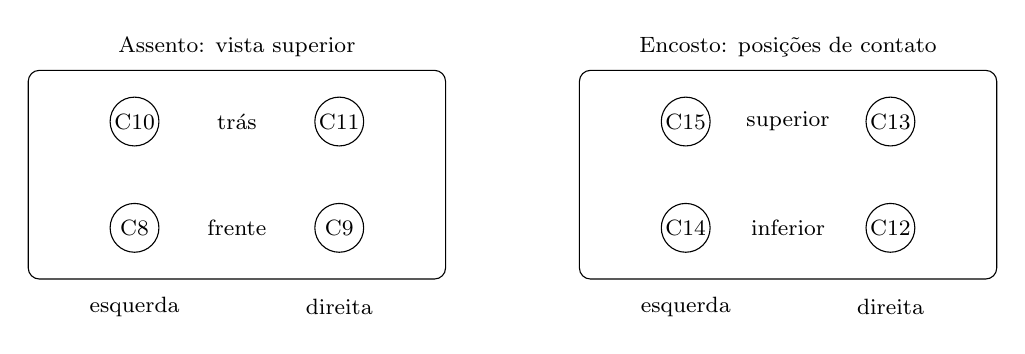
\begin{tikzpicture}[font=\footnotesize,
  s/.style={draw,circle,minimum size=.62cm,inner sep=0pt},
  t/.style={align=center}]
  \draw[rounded corners] (0,0) rectangle (5.3,2.65);
  \node at (2.65,2.95) {Assento: vista superior};
  \node[s] at (1.35,.65) {C8}; \node[s] at (3.95,.65) {C9};
  \node[s] at (1.35,2) {C10}; \node[s] at (3.95,2) {C11};
  \node[t] at (2.65,.65) {frente}; \node[t] at (2.65,2) {trás};
  \node at (1.35,-.35) {esquerda}; \node at (3.95,-.35) {direita};
  \begin{scope}[xshift=7cm]
   \draw[rounded corners] (0,0) rectangle (5.3,2.65);
   \node at (2.65,2.95) {Encosto: posições de contato};
   \node[s] at (1.35,.65) {C14}; \node[s] at (3.95,.65) {C12};
   \node[s] at (1.35,2) {C15}; \node[s] at (3.95,2) {C13};
   \node[t] at (2.65,.65) {inferior}; \node[t] at (2.65,2) {superior};
   \node at (1.35,-.35) {esquerda}; \node at (3.95,-.35) {direita};
  \end{scope}
 \end{tikzpicture}
 \end{SingleSpace}
 \fonte{Elaborado pelos autores (2026)}
 \label{fig:met-layout}
\end{figure}

O multiplexador CD74HC4067 seleciona os canais C8--C15 para a entrada
A0 \cite{ti_cd74hc4067}. Há um único pull-down de 3{,}3\,k\ohm{} em SIG,
compartilhado entre os canais. O caminho é 3{,}3\,V--FSR--multiplexador--SIG--
resistor--GND. Incluindo a resistência de condução $R_{\mathrm{on}}$,
\begin{equation}
 V_{\mathrm{SIG}}=V_{\mathrm{DD}}
 \frac{R_{\mathrm{fixo}}}{R_{\mathrm{fixo}}+R_{\mathrm{FSR}}+R_{\mathrm{on}}}.
 \label{eq:met-divisor}
\end{equation}
A tensão aumenta com a carga. Escolheu-se
$R_{\mathrm{fixo}}\approx\sqrt{R_{\min}R_{\max}}$ na faixa de contato de
interesse, como compromisso de resolução. O valor de 3{,}3\,k\ohm{} também
limita a corrente no sensor. O efeito fixo de $R_{\mathrm{on}}$ por canal
é incorporado à calibração individual.

O ADC tem resolução de 12 bits. A cada 50\,ms varrem-se os oito canais:
após cada seleção, aguardam-se 50\,$\mu$s, descarta-se a primeira conversão
e conserva-se a seguinte. O rádio é atendido entre canais para não atrasar
o ACK; a Figura~\ref{fig:met-fluxo-cadeira} representa esse escalonamento.
O botão de calibração conecta D9 ao GND, com pull-up interno e debounce
de 25\,ms. A cadeira utiliza a mesma topologia LiPo/USB do colar, mas seu
programa não implementa o monitor de corte nem o watchdog do vestível.

\begin{figure}[H]
 \centering
 \caption{Ciclo da cadeira, com atendimento frequente do rádio.}
 \begin{SingleSpace}
 \begin{tikzpicture}[
  b/.style={draw,rounded corners,font=\footnotesize,align=center,
   text width=3.55cm,minimum height=.8cm,inner sep=3pt},
  a/.style={-{Latex[length=1.7mm]},thick}]
  \node[b] (scan) at (0,0) {Varrer FSRs a 20\,Hz;\\atender rádio entre canais};
  \node[b] (cal) at (4.65,0) {Receber IMU; ler botão;\\calibrar quando solicitado};
  \node[b] (dec) at (9.3,0) {Se calibrado: aplicar fusão\\e portão temporal};
  \node[b] (ack) at (9.3,-1.8) {Preparar alerta e referência\\para o próximo ACK};
  \node[b] (out) at (4.65,-1.8) {Registrar CSV por USB;\\enviar beacon BLE};
  \node[b] (loop) at (0,-1.8) {Atualizar LED e enlace;\\repetir sem bloquear};
  \draw[a] (scan) -- (cal); \draw[a] (cal) -- (dec);
  \draw[a] (dec) -- (ack); \draw[a] (ack) -- (out);
  \draw[a] (out) -- (loop); \draw[a] (loop) -- (scan);
 \end{tikzpicture}
 \end{SingleSpace}
 \fonte{Elaborado pelos autores (2026)}
 \label{fig:met-fluxo-cadeira}
\end{figure}

\section{Integração}
\label{sec:met-integracao}

A Figura~\ref{fig:met-arquitetura} reúne sensoriamento, decisão e atuação.
O enlace utiliza Nordic Enhanced ShockBurst (ESB), pela biblioteca
\texttt{nrf\_to\_nrf}, com confirmação e retransmissão
\cite{nordic_esb,tmrh20_nrftonrf}. O colar transmite a orientação; a cadeira
prepara a decisão após a amostra $N$ e a devolve no payload do ACK de
$N+1$, em operação regular. Após 1\,s sem ACK de controle válido, o colar
usa a última referência recebida e aplica somente a regra inercial
(10\degree{}/3\,s, liberação abaixo de 7\degree{}). Sem referência, não alerta.

\begin{figure}[H]
 \centering
 \caption{Arquitetura autônoma e interfaces de acompanhamento.}
 \begin{SingleSpace}
 \begin{tikzpicture}[
  b/.style={draw,rounded corners,align=center,font=\footnotesize,
   text width=3.4cm,minimum height=.8cm,inner sep=3pt},
  a/.style={-{Latex[length=1.7mm]},thick},
  n/.style={font=\footnotesize,align=center,fill=white,inner sep=2pt}]
  \node[b] (imu) at (0,0) {Acelerômetro\\LSM6DS3TR-C};
  \node[b] (body) at (4.65,0) {XIAO do colar\\aquisição e atuação};
  \node[b] (motor) at (9.3,0) {BC337 + motor\\retorno vibratório};
  \node[b] (fsr) at (0,-2.3) {8 FSR402\\+ CD74HC4067};
  \node[b] (chair) at (4.65,-2.3) {XIAO da cadeira\\calibração e fusão};
  \node[b] (pc) at (9.3,-2.3) {Painel \texttt{mostra.py}\\USB / beacon BLE};
  \draw[a] (imu) -- node[n,above] {I\textsuperscript{2}C} (body);
  \draw[a] (body) -- node[n,above] {PWM} (motor);
  \draw[a] (fsr) -- node[n,above] {ADC} (chair);
  \draw[a] (body.south west) -- node[n,left] {ESB: ângulos\\20\,Hz} (chair.north west);
  \draw[a] (chair.north east) -- node[n,right] {ACK: alerta\\e referência} (body.south east);
  \draw[a] (chair) -- (pc);
 \end{tikzpicture}
 \end{SingleSpace}
 \fonte{Elaborado pelos autores (2026)}
 \label{fig:met-arquitetura}
\end{figure}

A calibração é individual, acionada pelo botão com o usuário ereto e
sentado até o fundo. Em 20 amostras válidas (cerca de 1\,s), calculam-se as
médias $p_0$, $r_0$ e $b_i$, referência angular e linha de base de cada FSR.
Falha inercial ou perda de enlace aborta a captura. Recusa-se a referência
se a soma traseira $B_T=b_{TE}+b_{TD}$ for inferior a 1000 contagens,
preservando a anterior. A referência fica em memória volátil e deve ser
refeita após reinício ou recolocação do colar. Durante a captura, as
decisões ficam suspensas e o LED verde pisca.

Na fusão, $FE$, $FD$, $TE$ e $TD$ indicam frente/trás e esquerda/direita
do assento. Os canais do encosto são registrados e exibidos, mas não
participam diretamente da decisão final, pois podem permanecer sem carga
mesmo na referência. Com leituras atuais $f_i$, definem-se
\begin{equation}
 \begin{gathered}
 \Delta p=p-p_0,\quad \Delta r=r-r_0,\quad
 d=\sqrt{\Delta p^2+\Delta r^2},\\
 S=f_{FE}+f_{FD}+f_{TE}+f_{TD},\qquad
 \rho=\frac{f_{TE}+f_{TD}}{B_T},\\
 \ell=\frac{f_{FE}+f_{TE}-f_{FD}-f_{TD}}{S}
      -\frac{b_{FE}+b_{TE}-b_{FD}-b_{TD}}{\sum_{i\in\mathrm{assento}}b_i}.
 \end{gathered}
 \label{eq:met-indicadores}
\end{equation}
A razão $\rho$ expressa o apoio traseiro relativo à referência; $\ell$
mede seu deslocamento lateral, positivo à esquerda. Define-se $h=\ell$
para $\Delta p<0$ e $h=-\ell$ nos demais casos, exigindo concordância com
a IMU. O termo lateral só é habilitado com base total do assento de pelo
menos 2000 contagens. O teste de vazio precede as divisões por $S$.

Com $\Delta r>0$ e $\rho\geq0{,}7$, considera-se reclinação apoiada:
usa-se $d_{\mathrm{ef}}=|\Delta p|$; nos demais casos,
$d_{\mathrm{ef}}=d$. Assim, preserva-se a avaliação lateral sem alertar
apenas pela inclinação para trás com apoio. A
Figura~\ref{fig:met-fusao} apresenta a ordem dos testes. Não há alerta
específico por pernas cruzadas; desvios do tronco ou escorregamento
continuam sendo avaliados.

\begin{figure}[H]
 \centering
 \caption{Prioridade da regra de fusão e encaminhamento ao portão temporal.}
 \begin{SingleSpace}
 \begin{tikzpicture}[y=1.4cm,
  q/.style={draw,align=center,font=\footnotesize,text width=5.3cm,
    minimum height=.65cm,inner sep=3pt},
  r/.style={draw,rounded corners,align=center,font=\footnotesize,
    text width=4.45cm,minimum height=.65cm,inner sep=3pt},
  a/.style={-{Latex[length=1.7mm]},thick},
  n/.style={font=\footnotesize,fill=white,inner sep=1pt}]
  \node[q] (invalid) at (0,0) {IMU inválida?};
  \node[q] (empty) at (0,-1.05) {$S<2000$ contagens?};
  \node[q] (slump) at (0,-2.1) {$\rho<0{,}3$?};
  \node[q] (dev) at (0,-3.15) {$d_{\mathrm{ef}}>10\degree{}$?};
  \node[q] (lean) at (0,-4.2) {Base lateral válida, $|\Delta p|\geq5\degree{}$\\e $h\geq0{,}08$?};
  \node[q] (ok) at (0,-5.35) {\texttt{RECLINE\_OK} se reclinado e $d>10\degree{}$;\\\texttt{OK} nos demais casos};
  \node[r] (ri) at (7.2,0) {\texttt{INVALID}: zerar portão};
  \node[r] (re) at (7.2,-1.05) {\texttt{EMPTY}: zerar portão};
  \node[r] (rs) at (7.2,-2.1) {\texttt{SLUMP}: condição ruim};
  \node[r] (rd) at (7.2,-3.15) {\texttt{IMU\_DEV}: condição ruim};
  \node[r] (rl) at (7.2,-4.2) {\texttt{LEAN}: condição ruim};
  \node[r] (gate) at (7.2,-5.35) {Portão: ruim por 3\,s dispara;\\sem condição ruim e $d_{\mathrm{ef}}<7\degree{}$ limpa};
  \foreach \x/\y in {invalid/empty,empty/slump,slump/dev,dev/lean,lean/ok}
    \draw[a] (\x) -- node[n,right] {não} (\y);
  \foreach \x/\y in {invalid/ri,empty/re,slump/rs,dev/rd,lean/rl}
    \draw[a] (\x) -- node[n,above] {sim} (\y);
  \draw[a] (ok) -- (gate);
  \draw[a] (rs.east) -- ++(.5,0) |- (gate.east);
  \draw (rd.east) -- ++(.5,0); \draw (rl.east) -- ++(.5,0);
 \end{tikzpicture}
 \end{SingleSpace}
 \fonte{Elaborado pelos autores (2026)}
 \label{fig:met-fusao}
\end{figure}

A condição ruim deve persistir por 3\,s, mesmo que mude de motivo.
Sem condição ruim, a contagem reinicia; um alerta ativo só é liberado
quando também $d_{\mathrm{ef}}<7\degree{}$. Na faixa intermediária,
conserva-se o estado anterior. IMU inválida, assento vazio, perda de enlace
na cadeira e calibração aceita zeram o portão. Sem host USB, 10\,s de
assento vazio também apagam a referência. A Tabela~\ref{tab:met-constantes}
resume as constantes de engenharia do protótipo, não limites clínicos.

\begin{table}[H]
 \centering
 \begin{SingleSpace}
 \caption{Constantes da aquisição, calibração e detecção.}
 \footnotesize
 \begin{tabularx}{\linewidth}{@{}X l X l@{}}
  \toprule
  Parâmetro & Valor & Parâmetro & Valor \\
  \midrule
  Aquisição / calibração & 20\,Hz / 20 amostras & Perda de enlace & 1\,s \\
  Disparo / liberação & 10\degree{} / 7\degree{} & Permanência & 3\,s \\
  Escorregamento ($\rho$) & $<0{,}3$ & Reclinação ($\rho$) & $\geq0{,}7$ \\
  Inclinação lateral & $\geq5\degree{}$ & Confirmação lateral ($h$) & $\geq0{,}08$ \\
  Assento vazio ($S$) & $<2000$ cont. & Base traseira mínima & 1000 cont. \\
  \bottomrule
 \end{tabularx}
 \fonte{Elaborado pelos autores (2026)}
 \label{tab:met-constantes}
 \end{SingleSpace}
\end{table}

O painel \texttt{mostra.py} recebe o estado por USB ou beacon BLE
unidirecional e apresenta desvio, mapa dos oito sensores, tempo sentado
e alerta. O painel permite acompanhar a operação, enquanto a decisão e
a vibração independem do computador.
